\documentclass[11pt,a4paper]{article}

\usepackage[utf8]{inputenc}
\usepackage[T1]{fontenc}
\usepackage{amsmath,amssymb,amsthm}
\usepackage{mathtools}
\usepackage{booktabs}
\usepackage{hyperref}
\usepackage{cleveref}
\usepackage{listings}
\usepackage{xcolor}
\usepackage{tikz}
\usetikzlibrary{positioning,arrows.meta,shapes.geometric,calc,decorations.pathreplacing}
\usepackage[margin=1in]{geometry}
\usepackage{natbib}
\usepackage{enumitem}

% Theorem environments
\newtheorem{theorem}{Theorem}[section]
\newtheorem{definition}[theorem]{Definition}
\newtheorem{proposition}[theorem]{Proposition}
\theoremstyle{remark}
\newtheorem{remark}[theorem]{Remark}

% Math operators
\DeclareMathOperator{\Aut}{Aut}
\DeclareMathOperator{\SO}{SO}
\DeclareMathOperator{\SU}{SU}
\DeclareMathOperator{\Ima}{Im}
\DeclareMathOperator{\proj}{proj}
\newcommand{\Oct}{\mathbb{O}}
\newcommand{\Real}{\mathbb{R}}
\newcommand{\Comp}{\mathbb{C}}
\newcommand{\Quat}{\mathbb{H}}

% Code listing style
\definecolor{codebg}{gray}{0.96}
\definecolor{codegreen}{rgb}{0.0,0.5,0.0}
\lstdefinestyle{python}{
  backgroundcolor=\color{codebg},
  basicstyle=\ttfamily\small,
  keywordstyle=\color{blue},
  commentstyle=\color{codegreen},
  stringstyle=\color{red!70!black},
  language=Python,
  frame=single,
  framerule=0.4pt,
  xleftmargin=1em,
  xrightmargin=1em,
  breaklines=true,
  showstringspaces=false,
}

% Epistemic honesty environment
\newenvironment{epistemicnote}{%
  \medskip\noindent\textbf{Epistemic honesty note.}\itshape\space
}{%
  \medskip
}

\title{Self-Organizing Octonionic Tries:\\Algebraic Memory Without Gradient Descent}
\author{Antonio Escalera}
\date{March 2026\\[0.5em]\normalsize Working Draft}

\begin{document}
\maketitle

\begin{abstract}
We propose a self-organizing hierarchical memory structure in which octonionic algebra replaces gradient-based learning entirely. The structure, an \textbf{octonionic trie}, is a dynamically growing tree whose nodes are individual octonions. Routing through the trie is governed by Fano plane subalgebra decomposition, growth is triggered by the associator (a measure of algebraic incompatibility), updates are performed by octonionic composition, and consistency is verified via algebraic inversion. The trie monitors its own structural health through invariants derived from the algebra: compression efficiency, subalgebra decomposition cleanliness, composition error bounds, and prediction consistency.

The result is a memory system that organizes, grows, consolidates, and self-corrects using only the algebraic properties of the octonions, without weight matrices, loss functions, or backward passes. The octonionic algebra provides the routing structure (7 quaternionic subalgebras via the Fano plane), the novelty detection mechanism (the associator), the update rule (norm-preserving multiplication), the consistency check (algebraic inversion), and the structural health metrics (associator norms, composition error). These are typically five separate engineered components in conventional memory-augmented architectures; here they emerge from a single algebraic substrate.

This work builds on the mathematical foundations established in the companion thesis on octonionic neural networks~\citep{Escalera2026}, extending the algebraic framework from gradient-trained networks to self-organizing structures that operate without optimization.
\end{abstract}

\tableofcontents
\newpage

%% ====================================================================
\section{Introduction and Motivation}
\label{sec:intro}
%% ====================================================================

Memory-augmented neural architectures (Neural Turing Machines~\citep{Graves2014}, Differentiable Neural Computers~\citep{Graves2016}, Memory Networks~\citep{Weston2015}) address a fundamental limitation of feedforward networks: the inability to store and retrieve structured information beyond what is captured in fixed weight matrices. These architectures introduce external memory modules with learned read/write controllers, enabling the network to maintain and manipulate an explicit memory state.

However, existing memory architectures share a common design pattern: the memory structure (flat array, matrix, or graph) is fixed a priori, and a trained controller learns to use it. The controller is optimized via gradient descent, the memory layout is predetermined, and the system cannot grow or restructure its memory in response to the data it encounters.

This paper proposes a fundamentally different approach. Rather than training a controller to manage a fixed memory, we construct a memory that \emph{organizes itself} using the algebraic properties of the octonions. The memory is a tree (trie) whose nodes are individual octonions. The tree grows when it encounters novel structure, updates by algebraic composition, verifies its own consistency via inversion, and prunes itself when structure becomes redundant. No component of this system requires gradient-based optimization.

The key insight is that the octonionic algebra provides, through its intrinsic mathematical structure, all the mechanisms that memory-augmented architectures typically engineer separately:

\begin{enumerate}[nosep]
  \item \textbf{Routing} via Fano plane subalgebra decomposition (7 quaternionic channels).
  \item \textbf{Novelty detection} via the associator $[a,b,c] = (ab)c - a(bc)$.
  \item \textbf{Content update} via norm-preserving octonionic multiplication.
  \item \textbf{Consistency verification} via algebraic inversion ($x^{-1} = \bar{x}/\lvert x \rvert^2$).
  \item \textbf{Structural health monitoring} via associator norms, composition error, and subalgebra coherence.
\end{enumerate}

These five mechanisms are not independent modules bolted together; they are consequences of the same algebraic structure. This economy of mechanism is the central argument for the octonionic trie.

\subsection{Relationship to Companion Work}

This paper depends on and extends the foundations established in~\citet{Escalera2026}:
\begin{itemize}[nosep]
  \item \textbf{Algebraic foundations} (Sections 1--3 of the companion): Hurwitz's theorem, octonionic multiplication, the Fano plane, $G_2$ automorphisms, the density argument.
  \item \textbf{Reversibility thesis} (Section 2): Algebraic invertibility enabling backward reasoning. The octonionic trie uses inversion for consistency checking (``rumination'').
  \item \textbf{Numerical stability} (Phase 4 experimental results): Composition error bounds that determine the trie's maximum depth.
  \item \textbf{Associator and subalgebra analysis} (Phase 9): Whether the associator carries useful information and whether subalgebras specialize. These are prerequisites for the trie's routing and novelty detection mechanisms.
\end{itemize}

The companion thesis validates these properties for gradient-trained octonionic networks. This paper proposes that the same properties support a qualitatively different computational paradigm: self-organization without optimization.

%% ====================================================================
\section{The Associator as a Computational Primitive}
\label{sec:associator}
%% ====================================================================

The associator is the mathematical object that makes the octonionic trie possible. This section establishes its properties and computational interpretation in detail.

\subsection{Definition and Algebraic Properties}

\begin{definition}[Associator]
For three octonions $a, b, c \in \Oct$, the \textbf{associator} is defined as:
\begin{equation}
  [a, b, c] = (ab)c - a(bc).
\end{equation}
The associator is an octonion-valued trilinear form measuring the failure of associativity for a given triple.
\end{definition}

The associator satisfies the following properties:

\begin{enumerate}[nosep]
  \item \textbf{Total antisymmetry:} $[a,b,c] = -[b,a,c] = -[a,c,b] = -[c,b,a]$. Swapping any two arguments flips the sign. This means the associator is sensitive to the ordering of all three elements.

  \item \textbf{Alternativity:} $[a,a,b] = [a,b,b] = 0$ for all $a, b \in \Oct$. When any two arguments are equal, the associator vanishes. The algebra is ``alternative'' even though it is not associative.

  \item \textbf{Subalgebra characterization:} $[a,b,c] = 0$ if and only if $a$, $b$, and $c$ generate an associative subalgebra (i.e., they all lie within the same quaternionic subalgebra of~$\Oct$, or within $\Real$ or $\Comp$). A nonzero associator certifies that the three elements span structure across multiple subalgebras.

  \item \textbf{Continuity:} The associator is a continuous function of its arguments. Small perturbations of the inputs produce small changes in the associator. This means the transition from ``compatible'' (small associator) to ``incompatible'' (large associator) is gradual, not discontinuous.

  \item \textbf{Norm bound:} $\lvert [a,b,c] \rvert \leq 2\lvert a \rvert \lvert b \rvert \lvert c \rvert$. The associator norm is bounded by the product of the input norms. For unit octonions, the maximum associator norm is~2.
\end{enumerate}

\subsection{Computational Interpretation}

In the context of the octonionic trie, the associator answers a specific question: \emph{given a new input $x$, an existing child node $c$, and their parent node $n$, does $x$ belong in the same branch as $c$?}

\begin{itemize}[nosep]
  \item $\lvert [x, c, n] \rvert \approx 0$: The triple $(x, c, n)$ generates an associative subalgebra. The input $x$ is algebraically compatible with the existing child $c$ in the context of parent $n$. Grouping does not matter; $x$ can be composed with $c$ without ambiguity. \textbf{Route to $c$ and update.}

  \item $\lvert [x, c, n] \rvert \gg 0$: The triple spans multiple subalgebras. The input $x$ introduces structure that is algebraically incompatible with $c$ in the context of $n$. The order of composition matters substantially, meaning $x$ carries information that $c$'s branch cannot accommodate without distortion. \textbf{$x$ does not belong in this branch.}

  \item $\lvert [x, c_i, n] \rvert \gg 0$ for \emph{all} children $c_i$: The input is incompatible with every existing branch. It represents genuinely novel structure. \textbf{Candidate for new node creation.}
\end{itemize}

The associator norm is a continuous scalar, providing a graded signal rather than a binary decision. The threshold separating ``compatible'' from ``incompatible'' is a design parameter that may be adaptive (e.g., proportional to the mean associator norm observed at that node).

\subsection{The Associator vs.\ Inner Product}

A natural question is why the associator is preferable to simpler similarity measures (e.g., octonionic inner product $\langle x, c \rangle = \text{Re}(\bar{x}c)$) for routing decisions.

The inner product measures how aligned two octonions are as vectors in $\Real^8$. It is a pairwise measure that ignores the algebraic context in which the comparison occurs. The associator is a \emph{three-way} measure that captures the relationship between two elements \emph{in the context of a third} (the parent node). This context-sensitivity is precisely what routing in a trie requires: whether an input belongs with a child depends not just on the input-child similarity, but on how both relate to the parent.

Furthermore, the inner product is symmetric and exists in every algebra (including $\Real^8$ with no octonionic structure). The associator is antisymmetric, trilinear, and exists \emph{only} in non-associative algebras. It is the uniquely octonionic signal: the information that octonions carry and that quaternions, complex numbers, and reals cannot.

%% ====================================================================
\section{Architecture of the Octonionic Trie}
\label{sec:architecture}
%% ====================================================================

\subsection{Structure}

\begin{definition}[Octonionic Trie]
An \textbf{octonionic trie} $\mathcal{T}$ is a rooted tree in which:
\begin{itemize}[nosep]
  \item Each node $v$ stores a single octonion $o_v \in \Oct$.
  \item Each node has at most 7 children, corresponding to the 7 quaternionic subalgebras of~$\Oct$ defined by the Fano plane.
  \item The tree grows dynamically: nodes are created when new data is algebraically incompatible with all existing branches, and consolidated when branches become redundant.
\end{itemize}
\end{definition}

The branching factor of 7 is not a design choice; it is a consequence of the Fano plane structure. The octonion $\Oct$ contains exactly 7 quaternionic subalgebras, each defined by an oriented triple $(e_i, e_j, e_k)$ of imaginary basis units. These subalgebras overlap (each imaginary unit belongs to exactly 3 subalgebras), providing a rich, interconnected routing structure rather than a disjoint partition.

\begin{figure}[ht]
\centering
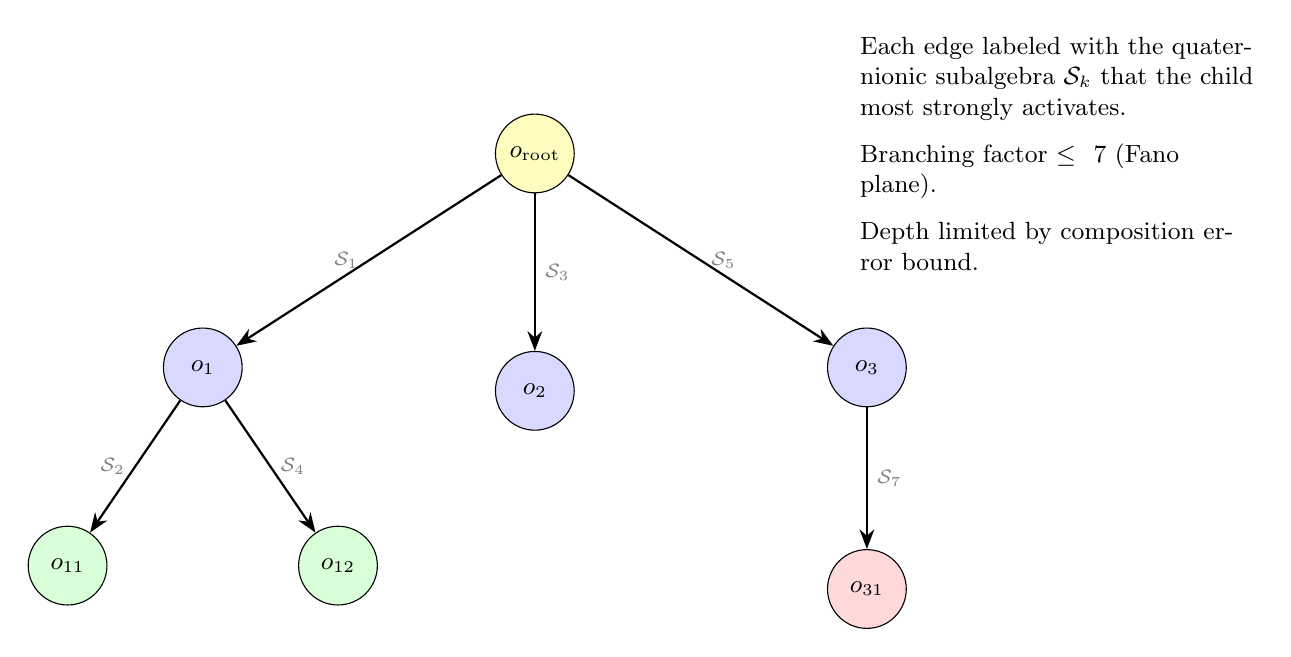
\begin{tikzpicture}[
    trienode/.style={circle, draw, fill=blue!15, minimum size=10mm, inner sep=0pt, font=\small},
    subalg/.style={font=\scriptsize\itshape, text=gray},
    edge/.style={thick, -{Stealth[length=2.5mm]}},
    level distance=2.2cm,
    sibling distance=2.8cm,
  ]
  % Root
  \node[trienode, fill=yellow!25] (root) {$o_{\text{root}}$};

  % Level 1
  \node[trienode, below left=2cm and 3.5cm of root] (c1) {$o_1$};
  \node[trienode, below=2cm of root] (c2) {$o_2$};
  \node[trienode, below right=2cm and 3.5cm of root] (c3) {$o_3$};

  % Level 2 (under c1)
  \node[trienode, fill=green!15, below left=1.8cm and 1cm of c1] (c11) {$o_{11}$};
  \node[trienode, fill=green!15, below right=1.8cm and 1cm of c1] (c12) {$o_{12}$};

  % Level 2 (under c3)
  \node[trienode, fill=red!15, below=1.8cm of c3] (c31) {$o_{31}$};

  % Edges
  \draw[edge] (root) -- node[subalg, left] {$\mathcal{S}_1$} (c1);
  \draw[edge] (root) -- node[subalg, right] {$\mathcal{S}_3$} (c2);
  \draw[edge] (root) -- node[subalg, right] {$\mathcal{S}_5$} (c3);
  \draw[edge] (c1) -- node[subalg, left] {$\mathcal{S}_2$} (c11);
  \draw[edge] (c1) -- node[subalg, right] {$\mathcal{S}_4$} (c12);
  \draw[edge] (c3) -- node[subalg, right] {$\mathcal{S}_7$} (c31);

  % Annotations
  \node[right=3.5cm of root, text width=5cm, font=\small] {
    Each edge labeled with the quaternionic subalgebra $\mathcal{S}_k$ that the child most strongly activates.\\[6pt]
    Branching factor $\leq 7$ (Fano plane).\\[6pt]
    Depth limited by composition error bound.
  };
\end{tikzpicture}
\caption{An octonionic trie with three levels. Each node stores a single octonion. Edges are labeled with the subalgebra activated by the child relative to its parent. Not all 7 children need to exist at each node; the trie grows on demand.}
\label{fig:trie}
\end{figure}

\subsection{Encoding: From Raw Data to Octonions}
\label{sec:encoding}

The octonionic trie operates on octonionic inputs. Raw data must be encoded into $\Oct$ before entering the trie. A key architectural property is that \textbf{the encoder is fully decoupled from the trie.}

The Fano plane subalgebra structure is a property of the octonionic multiplication table (the structure constants tensor $C_{ijk}$), not of the data or the encoding. When two octonions are multiplied and the result is decomposed along subalgebras, the decomposition is determined by $C_{ijk}$ regardless of how the octonions were produced. Consequently, the trie's self-organizing behavior is invariant to encoder quality: a better encoder produces richer octonionic representations, enabling the trie to capture more meaningful structure, but the trie's routing, growth, and consolidation mechanisms function identically for any encoder.

This decoupling has a practical consequence: any embedding model that produces dense vector representations (e.g., large language model embeddings, vision encoders, multimodal embeddings) can serve as the encoder, with a projection step mapping the embedding space into~$\Oct$.

\subsubsection{Hierarchical Projection}

A single linear projection from a high-dimensional embedding (e.g., $\Real^{768}$) to $\Oct$ ($\Real^8$) would discard most structure. However, the trie's tree structure provides a natural solution: \textbf{hierarchical decomposition.}

Rather than encoding the entire embedding into a single octonion, the encoding is distributed across trie levels:

\begin{itemize}[nosep]
  \item \textbf{Level 0:} A projection captures the coarsest structure of the embedding (e.g., the top 8 principal components). This determines the root-level routing.
  \item \textbf{Level $k$:} A projection captures the next level of detail, conditioned on the routing decisions at levels $0, \ldots, k-1$.
  \item \textbf{Cumulative representation:} A path of depth $k$ through the trie captures $8k$ effective dimensions of the original embedding, distributed across $k$ nodes.
\end{itemize}

The projections can be derived from principal component analysis of the embedding space: principal components 1--8 map to Level~0, components 9--16 to Level~1, and so on. This assignment is deterministic, requires no training, and naturally places the highest-variance (most discriminative) dimensions at the shallowest trie levels.

The trie's depth limit (determined by the composition error invariant, \cref{sec:invariants}) then corresponds to the maximum number of principal components the system can faithfully represent. This provides a principled, data-dependent capacity bound.

\begin{epistemicnote}
Whether PCA-based hierarchical projection preserves sufficient structure for routing to produce semantically meaningful trie organization is an empirical question. Alternative decompositions (independent component analysis, learned hierarchical projections) may perform better for specific data domains. The architectural claim is that the trie's self-organization is invariant to the choice of projection; the quality of the resulting organization is not.
\end{epistemicnote}

\subsection{Core Operations}
\label{sec:operations}

The octonionic trie supports four operations. None requires gradient computation.

\subsubsection{Compose: Routing and Update}

When a new input $x \in \Oct$ arrives, it is routed through the trie from root to leaf:

\begin{enumerate}[nosep]
  \item At each node $n$ with children $\{c_1, \ldots, c_k\}$, compute the octonionic product $p = n \cdot x$.
  \item Decompose $p$ along the 7 quaternionic subalgebras $\mathcal{S}_1, \ldots, \mathcal{S}_7$ of~$\Oct$.
  \item Select the child whose subalgebra has the largest projection: $c^* = \arg\max_i \lvert \proj_{\mathcal{S}_i}(p) \rvert$.
  \item Compute the associator $[x, c^*, n]$. If the norm is below the compatibility threshold, descend into $c^*$ and repeat.
  \item At the leaf, update the node by composition: $o_{\text{leaf}}' = o_{\text{leaf}} \cdot x$.
\end{enumerate}

The update step is norm-preserving when both operands are unit octonions ($\lvert ab \rvert = \lvert a \rvert \lvert b \rvert$). Sequential compositions do not cause the representation to explode or vanish.

The components of $p$ that fall outside the selected subalgebra constitute the \textbf{algebraic residual}. This residual is not discarded; it is recorded as metadata at the node (\cref{sec:residuals}).

\subsubsection{Detect: Novelty and Branching}

If the associator $[x, c_i, n]$ exceeds the compatibility threshold for \emph{all} existing children at a node, the input is flagged as a branching candidate. A branching event is not triggered immediately; persistent incompatibility across multiple inputs at the same node is required.

When a branching event is confirmed:
\begin{enumerate}[nosep]
  \item A new child node is created at the node $n$.
  \item The new child is initialized with the input $x$ (or a composition of the accumulated incompatible inputs).
  \item The new child is assigned to the subalgebra with the strongest residual accumulation (\cref{sec:residuals}), ensuring it occupies the region of octonionic space where the most unaccommodated structure has been observed.
\end{enumerate}

\subsubsection{Ruminate: Consistency Verification}

Before committing an update (composing $x$ into a leaf node), the trie verifies that the update is consistent with prior predictions that routed through the affected branch.

Each node maintains a bounded buffer of prior predictions (\cref{sec:memory}). The rumination procedure:
\begin{enumerate}[nosep]
  \item Tentatively compute the updated representation: $o' = o \cdot x$.
  \item For each buffered prediction $y$ that routed through this node, use algebraic inversion to estimate the counterfactual: ``If this node had been $o'$ instead of $o$, what would the prediction have been?''
  \item Compute the discrepancy between the original prediction and the counterfactual.
  \item If the maximum discrepancy exceeds the consistency threshold: reject the update and escalate to a branching decision. The input introduces structure that is inconsistent with the node's history.
  \item If all discrepancies are within threshold: commit the update.
\end{enumerate}

This is counterfactual reasoning enabled by algebraic invertibility. The system asks ``if I change my understanding here, do my past conclusions still hold?'' and acts on the answer.

\subsubsection{Consolidate: Pruning and Merging}

The trie periodically evaluates its structural health and consolidates:

\begin{itemize}[nosep]
  \item \textbf{Sibling absorption:} If a node has not been routed to recently (below a recency threshold), its representation is composed into its nearest sibling: $o_{\text{sibling}}' = o_{\text{sibling}} \cdot o_{\text{unused}}$. The unused node is removed. Because composition is invertible, the absorbed information is not destroyed but integrated into a more general representation.

  \item \textbf{Child merging:} If two children at a node have small pairwise associator ($\lvert [c_i, c_j, n] \rvert < \epsilon$), they are too similar to warrant separate branches. One is composed into the other and removed.

  \item \textbf{Depth limiting:} If the composition error at a given depth exceeds the scaling threshold (\cref{sec:invariants}), the node stops accepting new children. This branch has reached its representational resolution limit.
\end{itemize}

\subsection{Algebraic Residuals}
\label{sec:residuals}

When an input is routed to a specific child via subalgebra decomposition, the components of the octonionic product that fall in other subalgebras are the \textbf{algebraic residual}. These are not discarded but serve as metadata:

\begin{itemize}[nosep]
  \item A running mean direction (unit octonion) is maintained per unoccupied subalgebra at each node.
  \item A count of inputs contributing to each residual direction is tracked.
  \item When a branching event occurs (\cref{sec:operations}), the residual history informs the orientation of the new child: the subalgebra with the strongest accumulated residual is the natural location for the new branch.
\end{itemize}

Residuals are informational, not decisional. They record ``what structure has been observed but not accommodated'' without triggering any action. They answer the question ``if we ever need to branch here, where should the new child go?'' The associator remains the sole trigger for branching decisions.

\subsection{Memory Buffer and Relevance}
\label{sec:memory}

Each node (or each branch, defined as the path from root to a given node) maintains a bounded buffer of prior predictions for use in rumination (\cref{sec:operations}).

The buffer operates as follows:
\begin{itemize}[nosep]
  \item \textbf{Capacity:} Fixed-size ring buffer. Recent predictions are always retained.
  \item \textbf{Relevance filtering:} When an input arrives at a node, buffered predictions are scored for relevance. The relevance metric (octonionic inner product, norm-based similarity, or other measures) determines which memories are consulted during rumination. Predictions below a relevance threshold are skipped, bounding computation.
  \item \textbf{Percolation:} When a leaf makes a prediction, it is added to the buffers of all ancestor nodes along its branch. This ensures that consistency checks at any level of the trie have access to predictions from the entire subtree.
\end{itemize}

This memory model mirrors aspects of human memory: recent events are immediately accessible (ring buffer), and strongly relevant past experiences surface during familiar situations (relevance filtering). The octonionic algebra provides a natural relevance metric through the inner product $\langle x, y \rangle = \text{Re}(\bar{x}y)$, though whether this is the optimal metric for relevance is an empirical question.

%% ====================================================================
\section{Structural Invariants}
\label{sec:invariants}
%% ====================================================================

The octonionic trie monitors its own structural health through five invariants derived from the algebra. These invariants replace the role that loss functions play in gradient-trained systems.

\subsection{Composition Error Bound}

After composing $k$ inputs into a single node via sequential octonionic multiplication, floating-point error accumulates. The trie tracks:
\begin{equation}
  \varepsilon(d) = \frac{\lvert x^{-1} \cdot (o \cdot x) - o \rvert}{\lvert o \rvert}
\end{equation}
where $o$ is the node's representation and $x$ is the most recent input. When $\varepsilon(d)$ exceeds a threshold at depth $d$, the node stops growing deeper. This invariant establishes the trie's resolution limit per branch, connecting directly to the numerical stability characterization from Phase~4 of the companion thesis.

Different branches may have different depth limits depending on how cleanly their content decomposes along subalgebras. Branches with strong subalgebra alignment (small associators) accumulate error more slowly and can grow deeper.

\subsection{Compression Efficiency}

The trie monitors the ratio of structural complexity to prediction quality:
\begin{equation}
  \rho = \frac{\text{number of nodes}}{\text{effective prediction capacity}}.
\end{equation}
If a subtree has many nodes but contributes minimally to prediction quality (measured by how often its nodes are consulted during routing), the subtree is a candidate for consolidation. This is the minimum description length (MDL) principle applied structurally rather than as an optimization objective.

\subsection{Subalgebra Decomposition Cleanliness}

At each internal node, the pairwise associators between children measure how distinct the branches are:
\begin{equation}
  \text{cleanliness}(n) = \min_{i \neq j} \lvert [c_i, c_j, n] \rvert.
\end{equation}
High cleanliness means the children occupy genuinely different subalgebras and the branching is justified. Low cleanliness means the children are algebraically similar and should be considered for merging.

\subsection{Prediction Consistency}

The maximum discrepancy observed during rumination across the memory buffer:
\begin{equation}
  \delta(n) = \max_{y \in \text{buffer}(n)} \lvert \text{counterfactual}(y, o') - \text{original}(y) \rvert.
\end{equation}
When $\delta(n)$ is persistently high, the node's representation is unstable (frequent updates that would invalidate prior predictions). This may indicate the node is attempting to represent fundamentally incompatible information and should be split.

\subsection{Associator Health}

The mean associator norm at each node, averaged over recent inputs:
\begin{equation}
  \alpha(n) = \frac{1}{K} \sum_{k=1}^{K} \lvert [x_k, c^*_k, n] \rvert,
\end{equation}
where $c^*_k$ is the selected child for input $x_k$. A persistently high $\alpha(n)$ means the node's children are not accommodating incoming data well. A persistently low $\alpha(n)$ means the routing structure is effective. Trends in $\alpha(n)$ can signal that the node needs restructuring before a branching event is triggered.

%% ====================================================================
\section{Properties of the Architecture}
\label{sec:properties}
%% ====================================================================

\subsection{No Gradient Computation Required}

The octonionic trie operates entirely through algebraic operations: multiplication, inversion, subalgebra projection, and associator computation. None of these requires differentiability or a backward pass. The trie's ``learning'' consists of:
\begin{itemize}[nosep]
  \item \textbf{Composition:} accumulating structure via octonionic products.
  \item \textbf{Growth:} creating nodes when the associator signals novelty.
  \item \textbf{Consolidation:} merging or absorbing nodes when invariants indicate redundancy.
  \item \textbf{Self-correction:} rejecting updates that fail consistency checks.
\end{itemize}

The only component that may require gradient-based training is the encoder that maps raw data into octonionic representations (\cref{sec:encoding}). Once data is in $\Oct$, the trie is self-organizing.

\subsection{Encoder Invariance of Trie Structure}

The trie's routing, growth, and consolidation mechanisms depend on the octonionic multiplication structure (the structure constants $C_{ijk}$), not on the encoder. The Fano plane subalgebras, the associator, and the composition rule are properties of $\Oct$ that apply identically to any octonionic input regardless of its provenance.

A consequence: the same trie architecture can be used with different encoders (text embeddings, vision features, sensor data) without modification. The encoder determines the semantic quality of the trie's organization; the algebra determines the organizational mechanism.

\subsection{Information Preservation}

Octonionic composition is norm-preserving ($\lvert ab \rvert = \lvert a \rvert \lvert b \rvert$) and invertible ($a^{-1}$ exists for all $a \neq 0$). In exact arithmetic, no information is destroyed by composition, and any composition can be undone. Consolidation (sibling absorption) composes rather than discards, preserving information at a coarser level of representation.

In finite-precision arithmetic, composition error accumulates (\cref{sec:invariants}), providing a natural resolution limit. The trie degrades gracefully: deeper nodes have progressively lower fidelity, and the scaling invariant prevents growth beyond the point where fidelity is inadequate.

\subsection{Natural Hierarchy}

The trie's tree structure encodes hierarchy explicitly: parent nodes represent more general concepts, leaf nodes represent specific instances. The depth at which an input is stored reflects its specificity: inputs that are resolved at shallow depths are general (they fit cleanly into coarse-grained branches), while inputs requiring deep traversal are specific (they require fine-grained subalgebra distinctions).

This hierarchy emerges from the data and the algebra, not from architectural prescription. The trie does not have predefined ``levels of abstraction''; abstraction levels arise from the subalgebra decomposition of the data itself.

%% ====================================================================
\section{Relationship to Existing Architectures}
\label{sec:related}
%% ====================================================================

\begin{table}[ht]
\centering
\caption{Comparison with existing memory-augmented architectures.}
\label{tab:comparison}
\begin{tabular}{@{}lcccc@{}}
\toprule
Property & NTM/DNC & SDM & HTM & Oct-Trie \\
\midrule
Memory structure  & Flat array       & Sparse distributed & Columnar  & Tree (trie) \\
Growth mechanism  & Fixed size       & Fixed size          & Fixed columns & Dynamic (associator) \\
Routing           & Learned attention & Hamming distance   & Spatial pooling & Subalgebra decomposition \\
Update rule       & Learned write    & Superposition      & Hebbian   & Algebraic composition \\
Consistency check & None             & None                & None      & Algebraic inversion \\
Training          & Backprop         & None                & Hebbian   & None (algebraic) \\
Pruning           & None             & Decay               & Decay     & Sibling absorption \\
Self-monitoring   & None             & None                & Anomaly   & 5 algebraic invariants \\
\bottomrule
\end{tabular}
\smallskip

\noindent\footnotesize NTM = Neural Turing Machine~\citep{Graves2014}; DNC = Differentiable Neural Computer~\citep{Graves2016}; SDM = Sparse Distributed Memory~\citep{Kanerva1988}; HTM = Hierarchical Temporal Memory~\citep{Hawkins2016}.
\end{table}

The octonionic trie shares individual features with existing architectures but combines them in a way that, to our knowledge, has not been proposed:

\textbf{Kanerva's Sparse Distributed Memory}~\citep{Kanerva1988} uses high-dimensional binary addresses for content-addressable storage. The octonionic trie replaces binary address matching with subalgebra decomposition, providing a richer routing signal (7 overlapping 3D subspaces vs.\ Hamming distance in a flat binary space).

\textbf{Hierarchical Temporal Memory}~\citep{Hawkins2016} uses columnar structure inspired by neocortical columns, with Hebbian-like learning. The octonionic trie replaces the columnar structure with the Fano plane and Hebbian updates with algebraic composition. Both share the principle of learning without backpropagation.

\textbf{Neural Turing Machines}~\citep{Graves2014} use learned read/write heads over a flat memory matrix. The octonionic trie replaces learned attention with algebraic routing and learned writes with algebraic composition, eliminating the need for gradient-based controller training. The NTM's flat memory becomes a dynamic tree.

%% ====================================================================
\section{Open Questions}
\label{sec:open}
%% ====================================================================

\subsection{Empirical Validation Prerequisites}

Three empirical questions must be answered before the octonionic trie can be implemented:

\begin{enumerate}
  \item \textbf{Subalgebra routing discriminability.} Does projecting an octonionic product onto the 7 Fano subalgebras produce a clean enough signal to route semantically related inputs to the same branches? This can be tested by encoding a dataset with known categories into $\Oct$, constructing products at trie nodes, and measuring whether within-category inputs consistently activate the same subalgebras.

  \item \textbf{Associator as novelty signal.} Does the associator norm reliably spike when a genuinely novel category appears in a data stream? This can be tested on a sequential classification task where category boundaries are known.

  \item \textbf{Composition depth vs.\ information retention.} After composing $k$ inputs into a single node via sequential octonionic multiplication, how much of each input's structure is recoverable via inversion? The companion thesis's Phase~4 stability data provides bounds for layer-wise composition, but sequential data composition has different error characteristics.
\end{enumerate}

\subsection{Geometric Embedding of the Trie}

The companion thesis investigates whether the octonionic state space should carry a hyperbolic metric (\cref{sec:intro}). For the octonionic trie, the question takes a specific form: should the trie's nodes live on a hyperboloid $H^7$, in a Poincar\'{e} ball $B^8$, or in flat $\Oct$?

The trie's tree structure already encodes hierarchy explicitly (parent-child relationships). Adding a hyperbolic metric would make the embedding space \emph{also} encode hierarchy, providing redundancy that may improve distance-based operations (relevance filtering, nearest-sibling identification for consolidation) but adds the re-projection problem identified in the companion thesis (Section~8.7).

Flat $\Oct$ with the norm encoding node confidence or weight is the simplest starting point. The trie structure provides hierarchy; the algebra provides routing. Whether a hyperbolic metric provides additional benefit is an empirical question that should be investigated after the flat-space trie is validated.

\subsection{Composition Order}

Octonionic multiplication is non-commutative: $a \cdot b \neq b \cdot a$ in general. The update rule $o' = o \cdot x$ (node composed with input) produces a different result from $o' = x \cdot o$ (input composed with node). The choice affects subalgebra activation patterns and associator behavior. Both orderings should be characterized empirically; the correct choice may depend on whether the trie is intended to emphasize the existing representation (left-multiply by node) or the new information (left-multiply by input).

\subsection{Adaptive Thresholds}

The compatibility threshold for the associator, the consistency threshold for rumination, and the error threshold for depth limiting are design parameters. Whether these should be:
\begin{itemize}[nosep]
  \item Global constants,
  \item Per-node adaptive values (e.g., proportional to the node's mean associator norm),
  \item Derived from the data distribution (e.g., percentiles of observed associator norms),
\end{itemize}
is an open question with significant impact on the trie's sensitivity to novelty and its growth rate.

\subsection{Relevance Metric for Memory Buffer}

The choice of relevance metric for the memory buffer (\cref{sec:memory}) affects which prior predictions are consulted during rumination. Candidates include the octonionic inner product $\langle x, y \rangle = \text{Re}(\bar{x}y)$, the octonionic norm of the difference $\lvert x - y \rvert$, and subalgebra-projected similarity. The optimal metric likely depends on the task and may itself be a learnable component, though this would reintroduce a gradient-trained element into an otherwise algebraic system.

%% ====================================================================
\section{Conclusion}
\label{sec:conclusion}
%% ====================================================================

The octonionic trie demonstrates that the algebraic properties of the octonions, specifically the Fano plane subalgebra structure, the associator, norm-preserving multiplication, and algebraic invertibility, are sufficient to construct a self-organizing hierarchical memory without gradient-based optimization.

The architecture replaces five typically-engineered components (routing, novelty detection, content update, consistency verification, structural health monitoring) with consequences of a single algebraic structure. This economy of mechanism is the central argument: not that the octonionic trie outperforms existing memory architectures on benchmarks (this is an empirical question not yet tested), but that the algebraic substrate provides a coherent, minimal foundation from which all necessary memory operations emerge.

The trie's relationship to the companion thesis on octonionic neural networks~\citep{Escalera2026} is complementary. The companion thesis validates whether octonionic representations provide advantages in gradient-trained networks. This paper proposes that the same algebraic properties support a qualitatively different computational paradigm. If both are validated, the implication is that the octonionic algebra is not merely a useful parameterization for neural networks, but a general-purpose computational substrate for structured knowledge representation and reasoning.

%% ====================================================================
\bibliographystyle{plainnat}
\bibliography{references}

\end{document}
